Transferring files should also preserve the anonymity of the two participating 
parties. The original idea for achieving this consisted of transferring the 
files along the same paths used for searching. This is not completely feasible 
as the search paths can have an arbitrary length and the resulted network 
congestion would be quite significant (similar to Tor).

The current idea involves the file provider randomly choosing a number of 
\textit{Rendezvous nodes} (or \textit{Drop Points}), where it will transfer 
chunks of the file. The addresses of these Drop Points are communicated to the 
file downloader by the means of the search reply message (figure 
\ref{fig:fig5}). The chunks of the file are encrypted using the Transfer Key 
sent using the search reply, because of the possibility of one of the Drop 
Points being controlled by an adversary. The number of Drop Points is chosen 
based on the size of the file and the configuration of the Drop Points. The 
value of 100 MiB was selected intuitively for the default maximum size of a 
chunk. The Drop Points are chosen from the pool of neighbors. If the file 
provider does not have enough neighbors, it may request more addresses from one 
of the DNL hosts. These new addresses will be used only for the current 
transfer and not added as neighbors.

At this point, the node which requested the file could just ask the Drop Points 
for the file chunks, but there is a Man-in-the-middle attack possibility to 
consider. If an adversary replied to a search request and offers to transfer 
the file, it could provide node controlled by him as Drop Points. If the victim 
accesses those Drop Points directly then its identity would be known to the 
attacker. The downloader does not access the Drop Points directly, but instead 
delegates the "lifting" of the file chunks to a number of randomly chosen 
nodes, called \textit{Lift Proxies}. The process of choosing Lift Proxies is 
almost identical to the process of choosing Drop Points. A Lift Proxy node can 
be configured to lift chunk of a maximum size. Figure \ref{fig:fig7} 
illustrates a file transfer process.

\begin{figure}
    \centering
    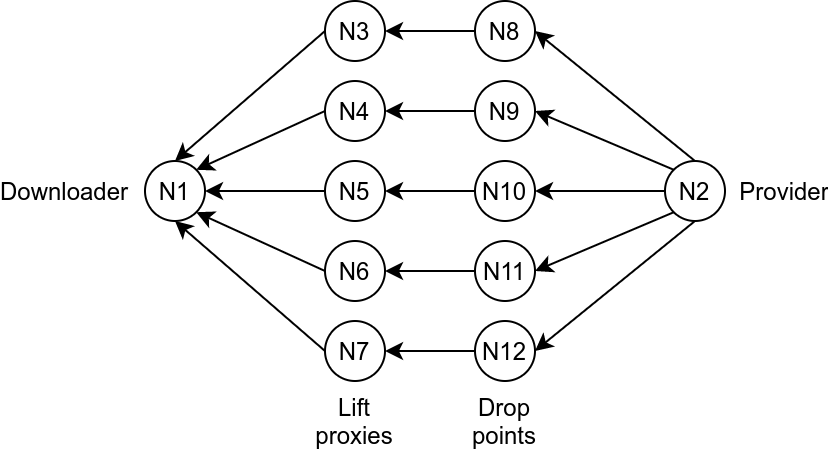
\includegraphics[width=0.6\textwidth]{figures/fig7}
    \caption{File transfer}
    \label{fig:fig7}
\end{figure}
